Escribe las expresiones algebraicas para cada una de las gr\'aficas en color de la figura \ref{fig:SINMAT1_U3_AC78_IMG1}.
\begin{figure}[H]
    \centering
    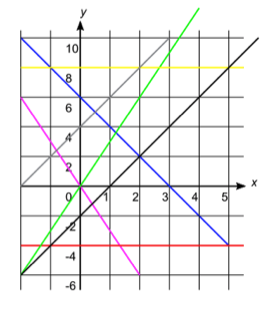
\includegraphics[width=0.4\textwidth]{../images/SINMAT1_U3_AC78_IMG1}
    \caption{Plano cartesiano con diferentes rectas distinguidas por colores.}
    \label{fig:SINMAT1_U3_AC78_IMG1}
\end{figure}

\begin{itemize}
    \item Recta negra: \fillin[$y = 2x - 2$][3cm]
    \item {\color{yellow} Recta amarilla}: \fillin[$y = 8$][3cm]
    \item {\color{green} Recta verde}: \fillin[$y = 3x$][3cm]
    \item {\color{gray} Recta gris}: \fillin[$y = 2x + 4$][3cm]
    \item {\color{blue} Recta azul}: \fillin[$y = -2x + 6$][3cm]
    \item {\color{purple} Recta violeta}: \fillin[$y = -3x $][3cm]
    \item {\color{red} Recta roja}: \fillin[$y = -4$][3cm]
\end{itemize}
